\documentclass[border=1pt]{standalone}
% Shared preamble for standalone figures in this directory.
% Compile with XeLaTeX from 讲义/figs, or via the figures target.
\usepackage{ctex}
\usepackage{amsmath}
\usepackage{amssymb}
\usepackage{bm}
\usepackage{mathtools}
\usepackage{tikz}
\renewcommand{\vec}[1]{\boldsymbol{#1}}
\newcommand{\cC}{\mathcal{C}}
\newcommand{\cD}{\mathcal{D}}
\newcommand{\R}{\mathbf{R}}
\usetikzlibrary{
    arrows.meta,
    calc,
    decorations.markings,
    angles,
    quotes,
    positioning,
    patterns,
    shapes.geometric
}

\begin{document}
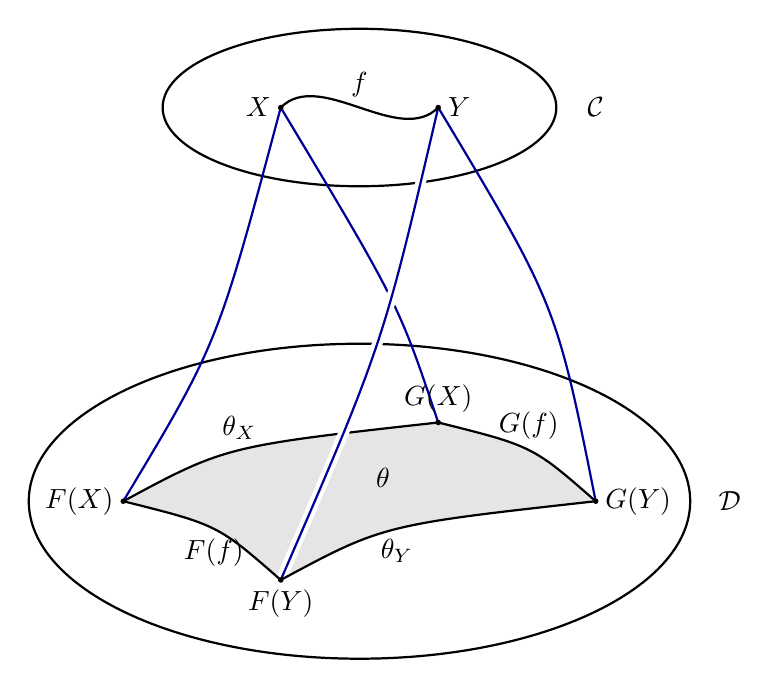
\begin{tikzpicture}
    \draw[thick] (0,3) ellipse (2.5 and 1)
    (0,-2) ellipse (4.2 and 2)
    node at (3, 3) {$\cC$}
    node at (4.7, -2) {$\cD$}
    coordinate (X) at (-1, 3)
    coordinate (Y) at (1, 3)
    coordinate (FX) at (-3, -2)
    coordinate (GY) at (3, -2)
    coordinate (GX) at (1, -1)
    coordinate (FY) at (-1, -3)
    coordinate (FX-GX-ct1) at (-1.7, -1.3)
    coordinate (FY-GY-ct1) at (0.3, -2.3)
    coordinate (FX-FY-ct1) at (-1.8, -2.3)
    coordinate (GX-GY-ct1) at (2.2, -1.3)
    coordinate (X-FX-ct1) at (-1.8, 0)
    coordinate (Y-FY-ct1) at (0.3, 0)
    coordinate (X-GX-ct1) at (0.5, 0.5)
    coordinate (Y-GY-ct1) at (2.5, 0.5);

    \fill[gray!20] (FX) .. controls (FX-GX-ct1) .. (GX) .. controls (GX-GY-ct1) .. (GY) .. controls (FY-GY-ct1) .. (FY) .. controls (FX-FY-ct1) .. (FX) -- cycle;

    \node at (0.3, -1.7) {$\theta$};

    \draw[thick] (FX) .. controls (FX-GX-ct1) .. node[above] {$\theta_X$} (GX) .. controls (GX-GY-ct1) .. node[above] {$G(f)$} (GY);
    \draw[thick,draw=blue!60!black] (X) .. controls (X-FX-ct1) .. (FX) (X) .. controls (X-GX-ct1) .. (GX);
    \draw[draw=white,double=blue!60!black,line width=1.5pt,double distance=0.8pt] (Y) .. controls (Y-FY-ct1) .. (FY);
    \draw[thick,draw=blue!60!black] (Y) .. controls (Y-GY-ct1) .. (GY);
    \draw[thick] (FX) .. controls (FX-FY-ct1) .. node[below] {$F(f)$} (FY) .. controls (FY-GY-ct1) .. node[below] {$\theta_Y$} (GY);
    \draw[thick] (X) .. controls (-.5, 3.5) and (.5, 2.5) .. node[above] {$f$} (Y);

    \node[left] at (X) {$X$};
    \node[right] at (Y) {$Y$};
    \node[left] at (FX) {$F(X)$};
    \node[right] at (GY) {$G(Y)$};
    \node[above] at (GX) {$G(X)$};
    \node[below] at (FY) {$F(Y)$};

    \foreach \point in {X, Y, FX, GX, GY, FY}
    \fill[black] (\point) circle (1pt);
\end{tikzpicture}

\end{document}
